\section{The $\pi_1$ Functor}

\begin{theorem}\label{4.2.1}
    The map $\pi_1:\Top \xrightarrow{} \Grp$ is a covariant functor. Moreover,
    if $h:(X,x_0) \xrightarrow{} (Y,y_0)$ and $k:(X,x_0) \xrightarrow{} (Y,y_0)$
    are continuous maps such that $h \simeq k \rel{x_0}$, then
    $\pi_1{h}=\pi_1{k}$.
\end{theorem}
\begin{proof}
    Let $[f] \in \pi_1(X,x_0)$ and define $\pi_1{h}:[f] \xrightarrow{} [h \circ
    f]$. Notice that the map $h \circ f:I \xrightarrow{} Y$ is continuous by
    composition and well defined. Moreover $h \circ f$ is a closed path in $Y$
    at $y_0$. This shows that $\pi_1{h}([f])=[h \circ f] \in \pi_1(Y,y_0)$. Now,
    if $f \simeq f' \rel{\partial{I}}$, then $h \circ f \simeq h \circ f'
    \rel{\partial{I}}$, so that if $f$ and  $g$ are closed paths in  $X$, at
    $x_0$, then $h\circ (f \ast g)=(h \circ f) \ast (h \circ g)$. This makes
    $\pi_1{h}$ into a homomorphism. Moreocer,
    $\pi_1{1_{(X,x_0)}}=1_{\pi_1(X,x_0)}$. This shows that $\pi_1$ is a functor,
    and that it is covariant.

    Now, let $h \simeq k \rel{\partial{I}}$. Then $h \circ f \simeq k \circ f
    \rel{\partial{I}}$, where $f$ is some closed path in $X$ at $x_0$. That is
    $\pi_1{h}=\pi_1{k}$.
\end{proof}

\begin{definition}
    We define the \textbf{pointed homotopy category} $\hTop$ to be the quotient
    category of $\Top^*$ arising from the congruence of relative homotopy.
\end{definition}

\begin{theorem}\label{4.2.2}
    Let $x_0 \in X$, and $X_0$ the path component of $X$ containing  $x_0$. Then
    $\pi_1(X_0,x_0) \simeq \pi_1(X,x_0)$.
\end{theorem}
\begin{proof}
    Consider the inclusion $j:(X_0,x_0) \xrightarrow{} (X,x_0)$ and let $[f] \in
    \ker{\pi_1{j}}$. Then $j \circ f \simeq c \rel{\partial{I}}$ where $c:I
    \xrightarrow{} X$ is the constant path from $t$ to  $x_0$. Let $F:j \circ f
    \simeq c$ a homotopy, then  $F(0,0)=x_0$, the space $F(I \times I)$ is path
    connected, and $F(I \times I) \subseteq X$. It remains to show that $f$ is
    nullhomotopic. Notice that  $F(I \times I)$ makes $\pi_1{j}$ 1--1. Now, if
    $f$ is a closed path in $X_0$ at $x_0$, then $f(I) \subseteq X_0$. Define
    $f':I \xrightarrow{} X_0$ by $f'(t)=f(t)$ for all $t \in I$. Then notice
    that  $j \circ f'=f$, this makes  $\pi_1{j}$ onto.
\end{proof}

\begin{theorem}\label{4.2.3}
    If $X$ is a path connected space, then the fundamental group of $X$ is
    independent of the basepoint chosen; i.e. if $x_0,x_1 \in X$, then
    $\pi_1(X,x_0) \simeq \pi_1(X,x_1)$.
\end{theorem}
\begin{proof}
    Let $\gamma:I \xrightarrow{} X$ be a path from $x_0$ to $x_1$. Define the
    map $\phi:\pi_1(X,x_0) \xrightarrow{} \pi_1(X,x_1)$ by $\phi:[f]
    \xrightarrow{} [\gamma][f][\inv{\gamma}]$. By theorem \ref{4.1.4}, $\phi$ is
    an isomorphism.
\end{proof}

\begin{definition}
    Let $H$ and  $K$ be sets. We define the  \textbf{projections} $p:H \times K
    \xrightarrow{} H$ and $q:H \times K \xrightarrow{} K$ defined by $p:h \times
    k \xrightarrow{} h$ and $q:h \times k \xrightarrow{} k$. Additionally, for
    some set $L$, there exist maps $\alpha:L \xrightarrow{} H$ and $\beta:L
    \xrightarrow{} H$ such that the map $\alpha \times \beta:L \xrightarrow{} H
    \times K$ satisfies $p \circ (\alpha \times \beta)=\alpha$ and $q \circ
    (\alpha \times \beta)=\beta$.
    \[\begin{tikzcd}
        & {H \times K} \\
        H && K \\
        & L
        \arrow["p"', from=1-2, to=2-1]
        \arrow["q", from=1-2, to=2-3]
        \arrow["\beta"', from=3-2, to=2-3]
        \arrow["\alpha", from=3-2, to=2-1]
        \arrow["{\alpha \times \beta}", dashed, from=3-2, to=1-2]
    \end{tikzcd}\]
\end{definition}

\begin{theorem}\label{4.2.4}
    For pointed spaces $(X,x_0)$ and $(Y,y_0)$, we have that $\pi_1(X \times Y,
    x_0 \times y_0) \simeq \pi_1(X,x_0) \times \pi_1(Y,y_0)$.
\end{theorem}
\begin{proof}
    Let $p$ and  $q$ the projections of  $(X \times Y, x_0 \times y_0)$ onto
    $(X,x_0)$ and $(Y,y_0)$, respectively. Then $\pi_1{p} \times
    \pi_1{q}:\pi_1(X \times Y,x_0 \times y_0) \xrightarrow{} \pi_1(X,x_0) \times
    \pi_1(Y,y_0)$ is a homomorphism. If $f$ is a closed path, in  $X \times Y$
    at  $x_0 \times y_0$, then $\pi_1{p} \times \pi_1{q}([f])=[pf] \times [qf]$.
    Now, let $g$ be a closed path in  $X$ at  $x_0$ and $h$ a closed path in
    $Y$ at  $y_0$ and define $\theta:[g] \times [h] \xrightarrow{} [g \times
    h]$. Then $\theta$ is well defined and is the incerse of  $\pi_1{p} \times
    \pi_1{q}$.
\end{proof}

\begin{lemma}\label{4.2.5}
    Suppose that $F:\phi_0 \simeq \phi_1$ is a free homotopy, where $\phi_0:X
    \xrightarrow{} Y$ and $\phi_1:X \xrightarrow{} Y$ are continuous. Choose an
    $x_0 \in X$ and let $\lambda=F(x_0,t)$ the path in $Y$ from $\phi_0(x_0)$ to
    $\phi_0(x_0)$. Then there is a commutative diagram
    \[\begin{tikzcd}
        {\pi_1(X,x_0)} && {\pi_1(Y,\phi_1(x_0))} \\
        \\
        && {\pi_1(Y,\phi_0(x_0))}
        \arrow["{\pi_1{\phi_1}}", from=1-1, to=1-3]
        \arrow["\psi", from=1-3, to=3-3]
        \arrow["{\pi_1{\phi_0}}"', from=1-1, to=3-3]
    \end{tikzcd}\]
    where $\psi:[g] \xrightarrow{} [\lambda \ast g \ast \inv{\lambda}]$.
\end{lemma}
\begin{proof}
    Let $f:I \xrightarrow{} X$ a closed path at $X$ and define  $G:I \times I
    \xrightarrow{} Y$ by $t \times s \xrightarrow{} F(f(s),t)$. Then $G:\phi_0
    \circ f \simeq \phi_1 \circ f$. Consider the triangulations of the box $I
    \times I$
     \begin{figure}[h]
        \centering
        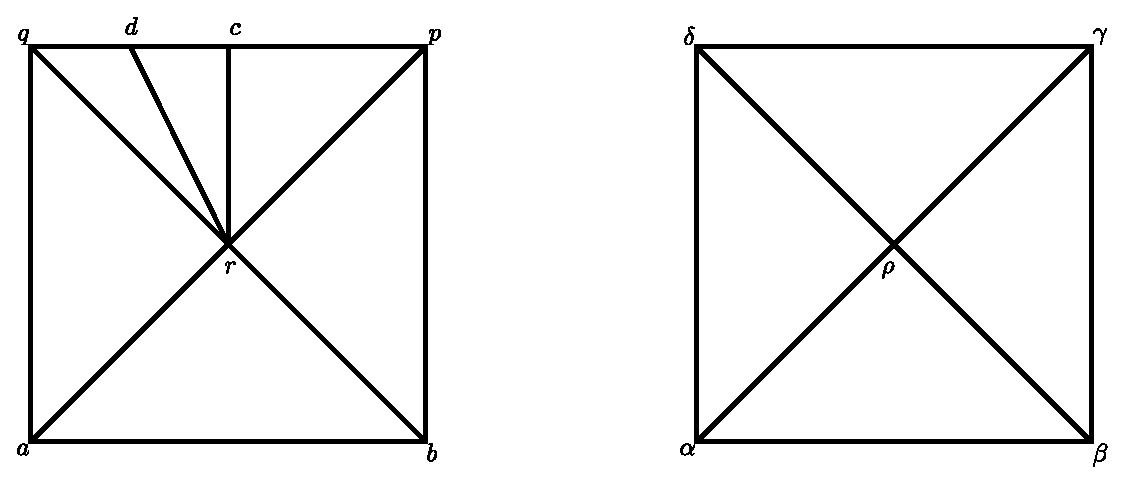
\includegraphics[scale=0.8]{Figures/Chapter4/affine_box.eps}
        \caption{}
        \label{}
    \end{figure}
    and define a continuous map $H:I \times I \xrightarrow{} I \times I$ by
    defining it in each triangle and applying the pasting lemma. Let
    \begin{align*}
        H(a)    &=  H(q)=\alpha \\
        H(b)    &=  H(p)=\beta \\
        H(c)    &=  \gamma \\
        H(d)    &=  \delta \\
        H(r)    &=  \rho \\
    \end{align*}
    Then the map $J=G \circ  H$ is a relative homotopy with  $J:\phi_0 \circ f
    \simeq \lambda \ast (\phi_1 \circ f) \ast \inv{\lambda} \rel{\partial{I}}$.
    So $\pi_1{\phi_0}([f])=[\phi_0 \circ f]=[\lambda \ast (\phi_1 \circ f) \ast
    \inv{\lambda}]$ and $\psi \circ \pi_1{\phi_1}([f])=\psi([\phi_1 \circ
f])=[\lambda \ast (\phi_1 \circ f) \ast \inv{\lambda}]$ as desired.
\end{proof}
\begin{corollary}
    If $\phi_0$ and $\phi_1$ are homotopic, then
    \begin{enumerate}
        \item[(1)] $\pi_1{\phi_0}$ and $\pi_1{\phi_1}$ are conjugate.

            \item[(2)] If $\pi_1(X,y_0)$ is Abelian, then
                $\pi_1{\phi_0}=\pi_1{\phi_1}$.
    \end{enumerate}
\end{corollary}

\begin{theorem}\label{4.2.6}
    If $\beta:X \xrightarrow{} Y$ is a homotopy equivalence, then the induces
    homomorphism $\pi_1{\beta}$ is an isomorphism for every $x_0 \in X$.
\end{theorem}
\begin{proof}
    Let $\alpha:Y \xrightarrow{} X$ a continuous map with $\alpha \circ
    \beta=1_X$ and  $\beta \circ \alpha=1_Y$. Then the lower triangle of the
    diagram
    \[\begin{tikzcd}
        & {\pi_1(Y,\beta(x_0))} \\
        {\pi_1(X,x_0)} && {\pi_1(X,\alpha \circ \beta(x_0))} \\
        & {\pi_1(X,x_0)}
        \arrow["{\pi_1{\beta}}", from=2-1, to=1-2]
        \arrow["{\pi_1{\alpha}}", from=1-2, to=2-3]
        \arrow["\psi", from=2-3, to=3-2]
        \arrow["1"', from=2-1, to=3-2]
        \arrow["{\pi_1{(\alpha \circ \beta)}}"{description}, from=2-1, to=2-3]
    \end{tikzcd}\]
    commutes. Since $\psi$, defined in lemma \ref{4.2.5} is an isomporphism,
    then so is $\pi_1{(\alpha \circ \beta)}$. Moreover, the top tirangle also
    commutes since $\pi_1$ is a functor, and $\pi_1{(\alpha \circ
    \beta)}=\pi_1{\alpha} \circ \pi_1{\beta}$, so that $\pi_1{\beta}$ is 1--1
    and $\pi_1{\alpha}$ is onto. A similar diagram arising from $\beta \circ
    \alpha=1_Y$ shows that  $\pi_1{\beta}$ is onto.
\end{proof}
\begin{corollary}
    If $X$ and  $Y$ are path connected with the same homotopy type, then for any
     $x_0 \in X$, $y_0 \in Y$, $\pi_1{(X,x_0)} \simeq \pi_1(Y,y_0)$.
\end{corollary}
\begin{corollary}
    If $X$ is a contractible space, then for any  $x_0 \in X$, $\pi_1(X,x_0)
    \simeq \langle 1 \rangle$, the trivial group.
\end{corollary}
\begin{corollary}
    If $\beta:(X,x_0) \xrightarrow{} (Y,y_0)$ is freely nullhomotopic, then the
    induced isomorphism $\pi_1{\beta}$ is trivial.
\end{corollary}
\begin{proof}
    Let $k:X \xrightarrow{} Y$ the constant map at $y$. Then  $\pi_1{k}$ is
    trivial since $\pi_1{k}([f])=[k \circ f]$ and $k \circ f$ is constant. Then
    if  $\beta \simeq k$ by lemma \ref{4.2.5}, there is an isomoprhism $\psi$
    with  $\psi \circ \pi_1{\beta}=\pi_1{k}$, so that
    $\pi_1{\beta}=\inv{\phi}\pi_1{k}$, which makes $\pi_1{\beta}$ trivial.
\end{proof}

\begin{definition}
    We call a topological space \textbf{simply connected} if it is path
    connected with trivial fundamental group.
\end{definition}
